% SPDX-License-Identifier: CC-BY-SA-4.0
% Copyright (c) 2026 Luis Alonso
%
% This file is part of luis_alonso/Notas-Japones.
%
% Licensed under Creative Commons Attribution-ShareAlike 4.0 International (CC BY-SA 4.0).
% You may share and adapt this material for any purpose,
% as long as you provide attribution and distribute adaptations under the same license.
%
% License: https://creativecommons.org/licenses/by-sa/4.0/
% Source:  https://git.lalonso.com/luis_alonso/Notas-Japones
%
% Note: Third-party content (if any) is excluded from this license and is marked where used.

\documentclass[a4paper,lualatex,ja=standard,base=10pt]{bxjsarticle}
\usepackage{setup}

\title{\ruby{第|０１|課}{だい||か} LV4}
\author{アロンゾ　ルイス}

\begin{document}
\setcounter{page}{1}

\maketitle{}
\thispagestyle{fancy}

\section{Repaso de nombres de familia}
\medskip

\subsection{Abuelos \ruby{祖|父|母}{そ|ふ|ぼ}}
\begin{VocabTable}[0.35\linewidth][→][P,P]
  \ruby{祖|父}{そ|ふ} & Abuelo (propio). \\
  おじいさん & Abuelo (otro). \\
  \ruby{祖|母}{そ|ぼ} & Abuela (propia). \\
  おばあさん & Abuela (otro). \\
\end{VocabTable}

\subsection{Padres \ruby{両|親}{りょう|しん}}
\begin{VocabTable}[0.35\linewidth][→][P,P]
  \ruby{父}{ちち} & Padre (propio). \\
  おとうさん & Padre (otro). \\
  \ruby{母}{はは} & Madre (propia). \\
  おかあさん & Madre (otro). \\
\end{VocabTable}

\subsection{Tíos \ruby{叔父|と|叔母}{おじ||おば}}
\begin{VocabTable}[0.35\linewidth][→][P,P]
  \ruby{叔父}{おじ} & Tío (propio). \\
  おじさん & Tío (otro). \\
  \ruby{叔母}{おば} & Tía (propia). \\
  おばさん & Tía (otro). \\
\end{VocabTable}

\subsection{Hermanos \ruby{兄弟}{きょうだい}}
\begin{VocabTable}[0.35\linewidth][→][P,P]
  \ruby{叔父}{おじ} & Tío (propio). \\
  おじさん & Tío (otro). \\
  \ruby{叔母}{おば} & Tía (propia). \\
  おばさん & Tía (otro). \\
\end{VocabTable}

\subsection{Hijos \ruby{子供}{こども}}
\begin{VocabTable}[0.35\linewidth][→][P,P]
  \ruby{息子}{むすこ} & Hijo (propio). \\
  むすこさん & Hijo (de otro). \\
  \ruby{娘}{むすめ} & Hija (propia). \\
  むすめさん & Hija (de otro). \\
\end{VocabTable}

\subsection{Esposo / Esposa \ruby{夫婦}{ふうふ}}
\begin{VocabTable}[0.35\linewidth][→][P,P]
  \ruby{夫}{おっと} & Esposo (propio). \\
  ご\ruby{主人}{しゅじん} & Esposo (de otro). \\
  \ruby{妻}{つま} & Esposa (propia). \\
  \ruby{奥様}{おくさま} & Esposa (de otro). \\
\end{VocabTable}

\section{Forma て}
\medskip

La forma て es una conjugación del verbo japonés que convierte el verbo en una
forma conectiva.

La forma て es una forma “puente” que conecta el verbo con otras ideas o
construcciones para dar funciones como secuencia, solicitud, permiso, etc.

\medskip

\subsection{１グループ Verbos que terminan con sonido イます}

\begin{figure}[H]
  \centering
  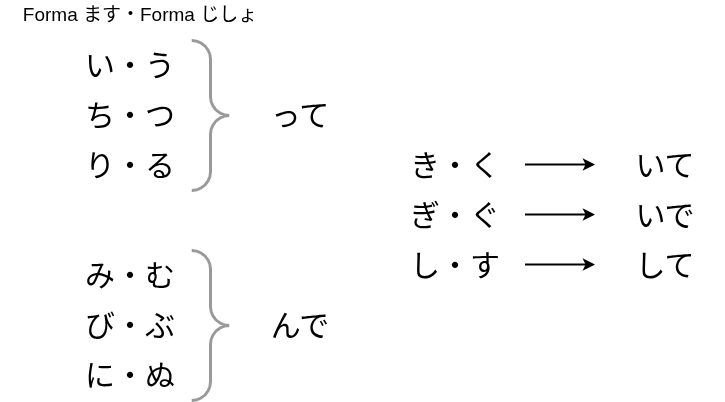
\includegraphics[width=0.6\linewidth]{assets/forma_te_1.png}
  \caption{Conversión de verbos del grupo 1}
\end{figure}

\begin{VocabTable}[0.35\linewidth][→][P,P]
  つくります & つく\textcolor{blue}{って}\\
  \ruby{行}{い}きます & \ruby{行}{い}\textcolor{blue}{って}\\
  \ruby{言}{い}います & \ruby{言}{い}\textcolor{blue}{いって}\\
  \ruby{泳}{およ}ぎます & \ruby{泳}{およ}\textcolor{blue}{いで}\\
  \ruby{話}{はな}します & \ruby{話}{はな}\textcolor{blue}{して}\\
  \ruby{待}{も}ちます & \ruby{待}{も}\textcolor{blue}{って}\\
  \ruby{死}{し}にます & \ruby{死}{し}\textcolor{blue}{んで}\\
  \ruby{遊}{あそ}びます & \ruby{遊}{あそ}\textcolor{blue}{んで}\\
\end{VocabTable}

\medskip
\subsection{２グループ Verbos que terminan en エます o tienen tres caracteres exactamente}

\begin{figure}[H]
  \centering
  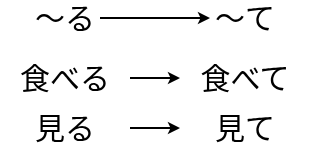
\includegraphics[width=0.4\linewidth]{assets/forma_te_2.png}
  \caption{Conversión de verbos del grupo 2}
\end{figure}

\begin{VocabTable}[0.35\linewidth][→][P,P]
  \ruby{食}{た}べます & \ruby{食}{た}べ\textcolor{blue}{て}\\
  あげます & あげ\textcolor{blue}{て}\\
  できます & でき\textcolor{blue}{て}\\
  \ruby{起}{お}きます & \ruby{起}{お}き\textcolor{blue}{て}\\
  \ruby{集}{あつ}めます & \ruby{集}{あつ}め\textcolor{blue}{て}\\
  います & い\textcolor{blue}{て}\\
\end{VocabTable}

\subsection{３グループ Verbos します/来ます y SUST+します}

\begin{figure}[H]
  \centering
  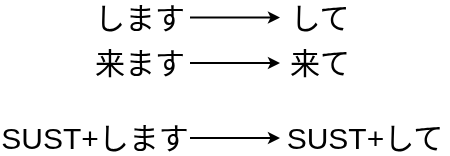
\includegraphics[width=0.4\linewidth]{assets/forma_te_3.png}
  \caption{Conversión de verbos del grupo 3}
\end{figure}


\begin{VocabTable}[0.35\linewidth][→][P,P]
  します & し\textcolor{blue}{て}\\
  \ruby{来}{き}ます & \ruby{来}{き}\textcolor{blue}{て}\\
  \ruby{勉強}{べんきょう}します & \ruby{勉強}{べんきょう}\textcolor{blue}{して}\\
  \ruby{運動}{うんどう}します & \ruby{運動}{うんどう}\textcolor{blue}{して}\\
  \ruby{掃除}{そうじ}します & \ruby{掃除}{そうじ}\textcolor{blue}{して}\\
  \ruby{運転}{うんてん}します & \ruby{運転}{うんてん}\textcolor{blue}{して}\\
\end{VocabTable}
\medskip

\section{Repaso de particulas}

に Se usa para:

\begin{itemize}
  \item Lugar donde.
  \item Indica direccion a donde se dirige.
\end{itemize}


で Se usa para:

\begin{itemize}
  \item Indicar como se ejecuta una accion.
  \item Lugar donde se realiza una accion.
  \item Herramienta con la cual se esta llevando acabo una accion.
\end{itemize}

\begin{VocabTable}[0.35\linewidth][→][P,P]
  Lugar + に + V & Indica lugar, hora exacta, dia exacto.\\
  Lugar + で + V & Lugar donde se realza accion.\\
  Medio + で + V & Indica en que medio se esta viajando.\\
  Idioma + で + V & Indica en que idioma se habla/escribe/lee.\\
\end{VocabTable}

% \section{Notas}
% \medskip
%
% 電車で、どのぐらいですか。 -> Cuanto tiempo te toma el tren.
%
% \subsection{Ejercicios}
%
% \begin{enumerate}
%   \item 私はコーヒーショップでおちゃを飲みます。
%   \item タクシーで学校に行きます。
%   \item \ruby{友|達}{とも|だち}と英語と中国語で話します。
%   \item フリアさんとホルヘさんはスペインにすんでいます。
% \end{enumerate}
%
% りかい P.26
%
% \begin{enumerate}
%   \item じてんしゃで/４０分ぐらい
%   \item あるいて/１５分ぐらい
%   \item 車/１時半
% \end{enumerate}
%
% りかい P.27
%
% \begin{enumerate}
%   \item に
%   \item で
%   \item に
%   \item で
%   \item で
%   \item に
% \end{enumerate}
%
% かつどう P.24
%
% \begin{enumerate}
%   \item a, 3, f
%   \item d, 4, i
%   \item b, 2, j
%   \item c, 6, h
% \end{enumerate}
%
% かつどう P.26
%
% まりさんのおねえさん
%
% \begin{itemize}
%   \item 日本語 <-
%   \item イタリア語
%   \item 英語 <-
% \end{itemize}
%
% まりさんのおにさん
%
% \begin{itemize}
%   \item 中国語 <-
%   \item 韓国語 <-
%   \item 日本語
% \end{itemize}
%
% まりさんのおばさん
%
% \begin{itemize}
%   \item 英語 <-
%   \item ポルトガル語
% \end{itemize}
%
% りかい P.28
%
% \begin{enumerate}
%   \item O
%   \item O
%   \item X
%   \item O
%   \item X
% \end{enumerate}
%
% \begin{enumerate}
%   \item 言います -> 言って
%   \item たちます -> たって
%   \item かえります -> かえって
%   \item 読みます -> 読んで
%   \item あそびます -> あそんで
%   \item しにます -> しんで
%   \item 書きます -> 書いて
%   \item ぬぎます -> ぬいで
%   \item 行きます -> 行って
%   \item 話します -> 話して
%   \item おきます -> おきて
%   \item できます -> できて
%   \item すがります -> すぐあって
%   \item まちがえって
%   \item りょうこして
%   \item おねがって
%   \item てつだって
%   \item つかって
%   \item おくれて
%   \item まって
%   \item 聴取て
%   \item もらって
%   \item くもって
%   \item 乗って
%   \item いて
% \end{enumerate}

\end{document}

